% answers.tex —— 2004 年·普通高等学校招生考试·浙江卷·理科 · 参考答案与详细解析片段
% 由 tools/generate_projects.py 依来源总账自 2004/2004_数学真题_浙江理科_试题.md + 2004/2004_数学真题_浙江理科_解析正文.md + 2004/2004_数学真题_浙江理科_答案要点.md 生成，勿手改（改源 MD 后重跑）


\begin{gktip}
固定源 PDF 为印刷页码 206–207 的两页题面，不附答案。以下解析均依据固定源独立推导复算；第 10 题三棱柱图、第 11 题导函数与四个候选图象图、第 19 题多面体图与第 22 题直角三角形中点折线图在 LaTeX 工程中以 TikZ 矢量源重绘。
\end{gktip}

\begin{answer}
\gksolhead{1}{}

\textbf{题目}：

若 $U = \{1, 2, 3, 4\}$，$M = \{1, 2\}$，$N = \{2, 3\}$，则 $\complement_U (M \cup N) =$\mbox{（　　）}

\begin{gkopts}(4)
\task A．$\{1, 2, 3\}$
\task B．$\{2\}$
\task C．$\{1, 3, 4\}$
\task D．$\{4\}$
\end{gkopts}

\Needspace{4\baselineskip}
\textbf{解析}

由已知条件，集合 $M = \{1, 2\}$，$N = \{2, 3\}$，
\Needspace{5\baselineskip}
所以两集合的并集为
\nopagebreak[4]
\[
M \cup N = \{1, 2, 3\}.
\]
\Needspace{5\baselineskip}
全集 $U = \{1, 2, 3, 4\}$，所以
\nopagebreak[4]
\[
\complement_U (M \cup N) = \{1, 2, 3, 4\} \setminus \{1, 2, 3\} = \{4\}.
\]
故选 D．

\gkanswer{答案：D}

\end{answer}
\begin{answer}
\gksolhead{2}{}

\textbf{题目}：

点 $P$ 从 $(1, 0)$ 出发，沿单位圆 $x^2 + y^2 = 1$ 逆时针方向运动 $\dfrac{2\pi}{3}$ 弧长到达 $Q$ 点，则 $Q$ 的坐标为\mbox{（　　）}

\begin{gkopts}(1)
\task A．$\left(-\dfrac{1}{2}, \dfrac{\sqrt{3}}{2}\right)$
\task B．$\left(-\dfrac{\sqrt{3}}{2}, -\dfrac{1}{2}\right)$
\task C．$\left(-\dfrac{1}{2}, -\dfrac{\sqrt{3}}{2}\right)$
\task D．$\left(-\dfrac{\sqrt{3}}{2}, \dfrac{1}{2}\right)$
\end{gkopts}

\Needspace{4\baselineskip}
\textbf{解析}

单位圆方程为 $x^2 + y^2 = 1$，其半径为 $r = 1$．
点 $P$ 从初始位置 $(1, 0)$ 出发，对应极角 $\theta_0 = 0$．
\Needspace{5\baselineskip}
沿逆时针方向运动弧长 $s = \dfrac{2\pi}{3}$，对应的圆心旋转角为
\nopagebreak[4]
\[
\Delta\theta = \frac{s}{r} = \frac{2\pi}{3}.
\]
\Needspace{5\baselineskip}
因此到达的终点 $Q$ 的坐标为
\nopagebreak[4]
\[
\left(\cos\frac{2\pi}{3}, \sin\frac{2\pi}{3}\right) = \left(-\frac{1}{2}, \frac{\sqrt{3}}{2}\right).
\]
故选 A．

\gkanswer{答案：A}

\end{answer}
\begin{answer}
\gksolhead{3}{}

\textbf{题目}：

已知等差数列 $\{a_n\}$ 的公差为 $2$，若 $a_1, a_3, a_4$ 成等比数列，则 $a_2 =$\mbox{（　　）}

\begin{gkopts}(4)
\task A．$-4$
\task B．$-6$
\task C．$-8$
\task D．$-10$
\end{gkopts}

\Needspace{4\baselineskip}
\textbf{解析}

设等差数列 $\{a_n\}$ 的首项为 $a_1$，已知公差 $d = 2$．
\Needspace{5\baselineskip}
由等差数列通项公式，
\nopagebreak[4]
\[
a_3 = a_1 + 2d = a_1 + 4, \quad a_4 = a_1 + 3d = a_1 + 6.
\]
\Needspace{5\baselineskip}
因为 $a_1, a_3, a_4$ 成等比数列，所以 $a_3^2 = a_1 a_4$，代入得
\nopagebreak[4]
\[
(a_1 + 4)^2 = a_1 (a_1 + 6),
\]
\Needspace{5\baselineskip}
展开整理得
\nopagebreak[4]
\[
a_1^2 + 8a_1 + 16 = a_1^2 + 6a_1 \implies 2a_1 = -16 \implies a_1 = -8.
\]
\Needspace{5\baselineskip}
所以
\nopagebreak[4]
\[
a_2 = a_1 + d = -8 + 2 = -6.
\]
故选 B．

\gkanswer{答案：B}

\end{answer}
\begin{answer}
\gksolhead{4}{}

\textbf{题目}：

曲线 $y^2 = 4x$ 关于直线 $x = 2$ 对称的曲线方程是\mbox{（　　）}

\begin{gkopts}(4)
\task A．$y^2 = 8 - 4x$
\task B．$y^2 = 4x - 8$
\task C．$y^2 = 16 - 4x$
\task D．$y^2 = 4x - 16$
\end{gkopts}

\Needspace{4\baselineskip}
\textbf{解析}

设所求对称曲线上任意一点的坐标为 $(x, y)$，其关于直线 $x = 2$ 的对称点为 $(x_0, y_0)$．
\Needspace{5\baselineskip}
由中点坐标公式，
\nopagebreak[4]
\[
\frac{x + x_0}{2} = 2 \implies x_0 = 4 - x, \quad y_0 = y.
\]
\Needspace{5\baselineskip}
因为点 $(x_0, y_0)$ 在原曲线 $y^2 = 4x$ 上，所以
\nopagebreak[4]
\[
y_0^2 = 4x_0,
\]
\Needspace{5\baselineskip}
代入得
\nopagebreak[4]
\[
y^2 = 4(4 - x) = 16 - 4x.
\]
故选 C．

\gkanswer{答案：C}

\end{answer}
\begin{answer}
\gksolhead{5}{}

\textbf{题目}：

设 $z = x - y$，式中变量 $x$ 和 $y$ 满足条件 $\begin{cases} x + y - 3 \geqslant 0, \\ x - 2y \geqslant 0, \end{cases}$ 则 $z$ 的最小值为\mbox{（　　）}

\begin{gkopts}(4)
\task A．$1$
\task B．$-1$
\task C．$3$
\task D．$-3$
\end{gkopts}

\Needspace{4\baselineskip}
\textbf{解析}

不等式组 $\begin{cases} x + y - 3 \geqslant 0, \\ x - 2y \geqslant 0 \end{cases}$ 表示的平面区域为：
边界直线 $x + y - 3 = 0$ 与 $x - 2y = 0$ 交于点 $A(2, 1)$．
可行域是由从点 $A(2, 1)$ 出发的两条射线所界定的无界区域，向 $x$ 轴正方向无限延伸．
目标函数为 $z = x - y$，即直线系方程 $y = x - z$．
直线的纵截距为 $-z$；当纵截距达到最大时，目标函数 $z$ 取得最小值．
直线 $x - 2y = 0$ 的斜率为 $\dfrac{1}{2}$，直线 $x + y - 3 = 0$ 的斜率为 $-1$．
目标函数直线的斜率为 $1 > \dfrac{1}{2} > -1$．
因此直线 $y = x - z$ 在可行域的交点顶点 $A(2, 1)$ 处取得最大纵截距，即 $z$ 取得最小值．
\Needspace{5\baselineskip}
代入点 $A(2, 1)$ 得
\nopagebreak[4]
\[
z_{\min} = 2 - 1 = 1.
\]
（亦可由 $y \leqslant \dfrac{1}{2}x$ 得 $z = x - y \geqslant x - \dfrac{1}{2}x = \dfrac{1}{2}x \geqslant \dfrac{1}{2} \times 2 = 1$ 直接获证）．
故选 A．

\gkanswer{答案：A}

\end{answer}
\begin{answer}
\gksolhead{6}{}

\textbf{题目}：

已知复数 $z_1 = 3 + 4\mathrm{i}$，$z_2 = t + \mathrm{i}$，且 $z_1 \cdot \overline{z_2}$ 是实数，则实数 $t =$\mbox{（　　）}

\begin{gkopts}(4)
\task A．$\dfrac{3}{4}$
\task B．$\dfrac{4}{3}$
\task C．$-\dfrac{4}{3}$
\task D．$-\dfrac{3}{4}$
\end{gkopts}

\Needspace{4\baselineskip}
\textbf{解析}

已知复数 $z_1 = 3 + 4\mathrm{i}$，$z_2 = t + \mathrm{i}$（$t \in \mathbf{R}$）．
\Needspace{5\baselineskip}
则 $z_2$ 的共轭复数为
\nopagebreak[4]
\[
\overline{z_2} = t - \mathrm{i}.
\]
\Needspace{5\baselineskip}
计算乘积：
\nopagebreak[4]
\[
z_1 \cdot \overline{z_2} = (3 + 4\mathrm{i})(t - \mathrm{i}) = 3t - 3\mathrm{i} + 4t\mathrm{i} - 4\mathrm{i}^2 = (3t + 4) + (4t - 3)\mathrm{i}.
\]
\Needspace{5\baselineskip}
因为 $z_1 \cdot \overline{z_2}$ 是实数，所以其虚部必须等于 $0$，即
\nopagebreak[4]
\[
4t - 3 = 0 \implies t = \frac{3}{4}.
\]
故选 A．

\gkanswer{答案：A}

\end{answer}
\begin{answer}
\gksolhead{7}{}

\textbf{题目}：

若 $\left(\sqrt{x} + \dfrac{2}{\sqrt[3]{x}}\right)^n$ 展开式中存在常数项，则 $n$ 的值可以是\mbox{（　　）}

\begin{gkopts}(4)
\task A．$8$
\task B．$9$
\task C．$10$
\task D．$12$
\end{gkopts}

\Needspace{4\baselineskip}
\textbf{解析}

\Needspace{5\baselineskip}
对于二项式 $\left(\sqrt{x} + \dfrac{2}{\sqrt[3]{x}}\right)^n$，其展开式的通项为
\nopagebreak[4]
\[
T_{r+1} = \mathrm{C}_n^r (\sqrt{x})^{n-r} \left(\frac{2}{\sqrt[3]{x}}\right)^r = \mathrm{C}_n^r 2^r x^{\frac{n-r}{2} - \frac{r}{3}} = \mathrm{C}_n^r 2^r x^{\frac{3n-5r}{6}},
\]
其中 $r \in \{0, 1, 2, \dots, n\}$．
\Needspace{5\baselineskip}
若展开式中存在常数项，则要求指数为 $0$：
\nopagebreak[4]
\[
\frac{3n - 5r}{6} = 0 \iff 3n = 5r \iff r = \frac{3n}{5}.
\]
因为 $r$ 必须为整数且 $0 \leqslant r \leqslant n$，又 $\gcd(3, 5) = 1$，所以正整数 $n$ 必须是 $5$ 的倍数．
在所给选项中：
\begin{gkopts}(1)
\task A．$8$ 不是 $5$ 的倍数；
\task B．$9$ 不是 $5$ 的倍数；
\task C．$10$ 是 $5$ 的倍数，此时 $r = 6 \in [0, 10]$ 为整数，存在常数项；
\task D．$12$ 不是 $5$ 的倍数．
\end{gkopts}
因此 $n$ 的值可以是 $10$．
故选 C．

\gkanswer{答案：C}

\end{answer}
\begin{answer}
\gksolhead{8}{}

\textbf{题目}：

在 $\triangle ABC$ 中，“$A > 30^\circ$”是“$\sin A > \dfrac{1}{2}$”的\mbox{（　　）}

\begin{gkopts}(2)
\task A．充分而不必要条件
\task B．必要而不充分条件
\task C．充分必要条件
\task D．既不充分也不必要条件
\end{gkopts}

\Needspace{4\baselineskip}
\textbf{解析}

在 $\triangle ABC$ 中，内角 $A \in (0, 180^\circ)$．
若 $A > 30^\circ$，取 $A = 150^\circ$，则 $\sin A = \sin 150^\circ = \dfrac{1}{2}$，不满足 $\sin A > \dfrac{1}{2}$；
取 $A = 160^\circ$，则 $\sin A = \sin 20^\circ < \dfrac{1}{2}$；
因此“$A > 30^\circ$”推不出“$\sin A > \dfrac{1}{2}$”，即不充分；
\Needspace{5\baselineskip}
反之，若 $\sin A > \dfrac{1}{2}$，由 $A \in (0, 180^\circ)$，解得
\nopagebreak[4]
\[
30^\circ < A < 150^\circ,
\]
显然在此范围内恒有 $A > 30^\circ$ 成立，故“$\sin A > \dfrac{1}{2}$”能推出“$A > 30^\circ$”，即必要．
综上，“$A > 30^\circ$”是“$\sin A > \dfrac{1}{2}$”的必要而不充分条件．
故选 B．

\gkanswer{答案：B}

\end{answer}
\begin{answer}
\gksolhead{9}{}

\textbf{题目}：

若椭圆 $\dfrac{x^2}{a^2} + \dfrac{y^2}{b^2} = 1$（$a > b > 0$）的左、右焦点分别为 $F_1$、$F_2$，线段 $F_1 F_2$ 被抛物线 $y^2 = 2bx$ 的焦点分成 $5 : 3$ 两段，则此椭圆的离心率为\mbox{（　　）}

\begin{gkopts}(2)
\task A．$\dfrac{16}{17}$
\task B．$\dfrac{4\sqrt{17}}{17}$
\task C．$\dfrac{4}{5}$
\task D．$\dfrac{2\sqrt{5}}{5}$
\end{gkopts}

\Needspace{4\baselineskip}
\textbf{解析}

椭圆 $\dfrac{x^2}{a^2} + \dfrac{y^2}{b^2} = 1$（$a > b > 0$）的左、右焦点分别为 $F_1(-c, 0)$、$F_2(c, 0)$，其中 $c = \sqrt{a^2 - b^2}$．
抛物线 $y^2 = 2bx$ 的焦点坐标为 $F\left(\dfrac{b}{2}, 0\right)$．
因为 $b > 0$，所以抛物线焦点 $F$ 位于 $x$ 轴正半轴上．
线段 $F_1 F_2$ 的端点坐标为 $-c$ 与 $c$．
\Needspace{5\baselineskip}
点 $F$ 将线段 $F_1 F_2$ 分为两段，其长度分别为
\nopagebreak[4]
\[
|F_1 F| = \frac{b}{2} - (-c) = c + \frac{b}{2}, \quad |F F_2| = c - \frac{b}{2}.
\]
因为 $b > 0$，显然 $|F_1 F| > |F F_2|$．
\Needspace{5\baselineskip}
由题意，两段长度之比为 $5 : 3$，即
\nopagebreak[4]
\[
\frac{c + \dfrac{b}{2}}{c - \dfrac{b}{2}} = \frac{5}{3}.
\]
\Needspace{5\baselineskip}
去分母整理得
\nopagebreak[4]
\[
3\left(c + \frac{b}{2}\right) = 5\left(c - \frac{b}{2}\right) \implies 3c + \frac{3}{2}b = 5c - \frac{5}{2}b \implies 2c = 4b \implies c = 2b.
\]
因此 $b = \dfrac{c}{2}$．
\Needspace{5\baselineskip}
代入椭圆关系式 $b^2 = a^2 - c^2$：
\nopagebreak[4]
\[
\frac{c^2}{4} = a^2 - c^2 \implies \frac{5}{4}c^2 = a^2.
\]
\Needspace{5\baselineskip}
两边除以 $a^2$：
\nopagebreak[4]
\[
\frac{5}{4}e^2 = 1 \implies e^2 = \frac{4}{5} \implies e = \frac{2}{\sqrt{5}} = \frac{2\sqrt{5}}{5}.
\]
故选 D．

\gkanswer{答案：D}

\end{answer}
\begin{answer}
\gksolhead{10}{}

\textbf{题目}：

如图，在正三棱柱 $ABC - A_1B_1C_1$ 中已知 $AB = 1$，$D$ 在棱 $BB_1$ 上，且 $BD = 1$，若 $AD$ 与平面 $AA_1C_1C$ 所成的角为 $\alpha$，则 $\alpha =$\mbox{（　　）}
\nopagebreak[4]
\begin{center}% Candidate source: src-e83c48821eaac4546df1607aa7bd47f8c49362fe9d091f3ff8accf356722e61c
% Source PDF SHA-256: 0a787b530b939cb104a802de2c27119b5d150bac7c4f0e78b069bc103f381232
% PDF page 1 (printed page 206), question 10.
% Redraw follows visible/hidden edges: regular triangular prism ABC-A1B1C1, point D on BB1, lines AD and C1A.
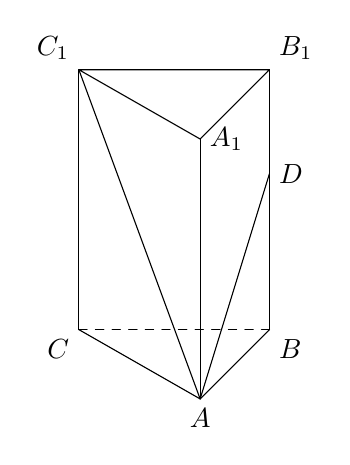
\begin{tikzpicture}[line cap=round,line join=round,>=latex,scale=1.1]
  % Bottom face vertices
  \coordinate (C) at (0,0);
  \coordinate (B) at (2.2,0);
  \coordinate (A) at (1.4,-0.8);

  % Top face vertices (vertical shift 3.0)
  \coordinate (C1) at (0,3.0);
  \coordinate (B1) at (2.2,3.0);
  \coordinate (A1) at (1.4,2.2);

  % Point D on BB1
  \coordinate (D) at (2.2,1.8);

  % Hidden edges
  \draw[dashed] (C) -- (B);

  % Visible edges: bottom face
  \draw (C) -- (A) -- (B);

  % Visible edges: top face
  \draw (C1) -- (A1) -- (B1) -- cycle;

  % Lateral edges
  \draw (C) -- (C1);
  \draw (B) -- (B1);
  \draw (A) -- (A1);

  % Connecting lines AD and C1A
  \draw (A) -- (D);
  \draw (C1) -- (A);

  % Vertex labels
  \node[below left] at (C) {$C$};
  \node[below right] at (B) {$B$};
  \node[below] at (A) {$A$};
  \node[above left] at (C1) {$C_1$};
  \node[above right] at (B1) {$B_1$};
  \node[right] at (A1) {$A_1$};
  \node[right] at (D) {$D$};
\end{tikzpicture}
\end{center}
\nopagebreak[4]
\begin{gkopts}(2)
\task A．$\dfrac{\pi}{3}$
\task B．$\dfrac{\pi}{4}$
\task C．$\arcsin\dfrac{\sqrt{10}}{4}$
\task D．$\arcsin\dfrac{\sqrt{6}}{4}$
\end{gkopts}

\Needspace{4\baselineskip}
\textbf{解析}
\nopagebreak[4]
\begin{center}% Candidate source: src-e83c48821eaac4546df1607aa7bd47f8c49362fe9d091f3ff8accf356722e61c
% Source PDF SHA-256: 0a787b530b939cb104a802de2c27119b5d150bac7c4f0e78b069bc103f381232
% PDF page 1 (printed page 206), question 10.
% Redraw follows visible/hidden edges: regular triangular prism ABC-A1B1C1, point D on BB1, lines AD and C1A.
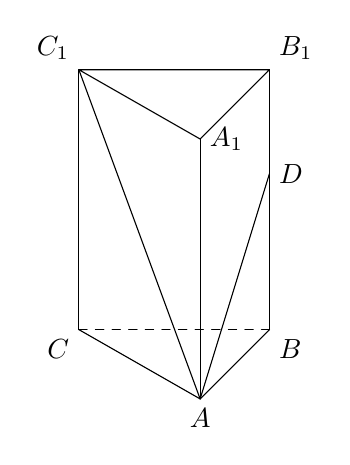
\begin{tikzpicture}[line cap=round,line join=round,>=latex,scale=1.1]
  % Bottom face vertices
  \coordinate (C) at (0,0);
  \coordinate (B) at (2.2,0);
  \coordinate (A) at (1.4,-0.8);

  % Top face vertices (vertical shift 3.0)
  \coordinate (C1) at (0,3.0);
  \coordinate (B1) at (2.2,3.0);
  \coordinate (A1) at (1.4,2.2);

  % Point D on BB1
  \coordinate (D) at (2.2,1.8);

  % Hidden edges
  \draw[dashed] (C) -- (B);

  % Visible edges: bottom face
  \draw (C) -- (A) -- (B);

  % Visible edges: top face
  \draw (C1) -- (A1) -- (B1) -- cycle;

  % Lateral edges
  \draw (C) -- (C1);
  \draw (B) -- (B1);
  \draw (A) -- (A1);

  % Connecting lines AD and C1A
  \draw (A) -- (D);
  \draw (C1) -- (A);

  % Vertex labels
  \node[below left] at (C) {$C$};
  \node[below right] at (B) {$B$};
  \node[below] at (A) {$A$};
  \node[above left] at (C1) {$C_1$};
  \node[above right] at (B1) {$B_1$};
  \node[right] at (A1) {$A_1$};
  \node[right] at (D) {$D$};
\end{tikzpicture}
\end{center}
\nopagebreak[4]
在正三棱柱 $ABC - A_1B_1C_1$ 中，底面 $\triangle ABC$ 为正三角形，边长 $AB = 1$；侧棱垂直于底面．
取 $AC$ 的中点为 $O$，连接 $BO$．
\Needspace{5\baselineskip}
在正三角形 $ABC$ 中，因为 $AB = BC = CA = 1$ 且 $O$ 为 $AC$ 中点，所以
\nopagebreak[4]
\[
BO \perp AC, \quad BO = \frac{\sqrt{3}}{2}AB = \frac{\sqrt{3}}{2}.
\]
\Needspace{5\baselineskip}
又因为侧棱 $AA_1 \perp$ 平面 $ABC$ 且 $BO \subset$ 平面 $ABC$，所以
\nopagebreak[4]
\[
BO \perp AA_1.
\]
\Needspace{5\baselineskip}
因为 $BO \perp AC$ 且 $BO \perp AA_1$，$AC \cap AA_1 = A$，所以
\nopagebreak[4]
\[
BO \perp \text{平面} AA_1C_1C.
\]
因为棱 $BB_1 \parallel AA_1$，所以 $BB_1 \parallel$ 平面 $AA_1C_1C$．
棱 $BB_1$ 上任意一点到平面 $AA_1C_1C$ 的距离均等于 $BO = \dfrac{\sqrt{3}}{2}$．
过点 $D$ 作 $DH \perp$ 平面 $AA_1C_1C$ 于点 $H$，则 $DH \parallel BO$，且 $DH = BO = \dfrac{\sqrt{3}}{2}$．
连接 $AH$，则 $AH$ 为直线 $AD$ 在平面 $AA_1C_1C$ 内的射影，
因此 $\angle DAH$ 即为直线 $AD$ 与平面 $AA_1C_1C$ 所成的角 $\alpha$．
\Needspace{5\baselineskip}
在 Rt$\triangle ABD$ 中，因为 $BB_1 \perp AB$，$AB = 1$，$BD = 1$，由勾股定理得
\nopagebreak[4]
\[
AD = \sqrt{AB^2 + BD^2} = \sqrt{1^2 + 1^2} = \sqrt{2}.
\]
\Needspace{5\baselineskip}
在 Rt$\triangle AHD$ 中，$\angle AHD = 90^\circ$，所以
\nopagebreak[4]
\[
\sin\alpha = \frac{DH}{AD} = \frac{\dfrac{\sqrt{3}}{2}}{\sqrt{2}} = \frac{\sqrt{6}}{4}.
\]
\Needspace{5\baselineskip}
因为 $\alpha \in \left(0, \dfrac{\pi}{2}\right)$，所以
\nopagebreak[4]
\[
\alpha = \arcsin\frac{\sqrt{6}}{4}.
\]
故选 D．

\gkanswer{答案：D}

\end{answer}
\begin{answer}
\gksolhead{11}{}

\textbf{题目}：

设 $f'(x)$ 是函数 $f(x)$ 的导函数，$y = f'(x)$ 的图象如图所示，则 $y = f(x)$ 的图象最有可能的是\mbox{（　　）}
\nopagebreak[4]
\begin{center}% Candidate source: src-e83c48821eaac4546df1607aa7bd47f8c49362fe9d091f3ff8accf356722e61c
% Source PDF SHA-256: 0a787b530b939cb104a802de2c27119b5d150bac7c4f0e78b069bc103f381232
% PDF page 1 (printed page 206), question 11.
% Redraw follows visible relations: derivative graph y = f'(x) and four candidate curves (A)–(D).
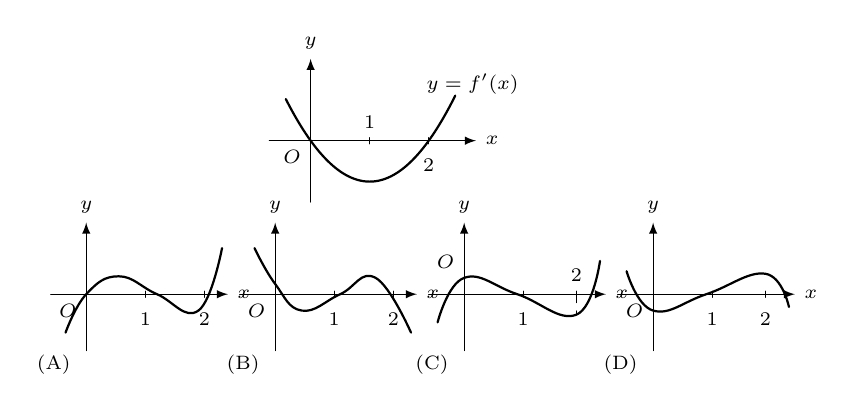
\begin{tikzpicture}[line cap=round,line join=round,>=latex,x=0.75cm,y=0.65cm,every node/.style={font=\scriptsize}]
  % Top: prompt curve y = f'(x)
  \begin{scope}[shift={(3.8,3.0)}]
    \draw[->] (-0.7,0) -- (2.8,0) node[right] {$x$};
    \draw[->] (0,-1.2) -- (0,1.6) node[above] {$y$};
    \node[below left] at (0,0) {$O$};
    \draw[thick,domain=-0.42:2.45,samples=80] plot (\x,{0.8*\x*(\x-2)});
    \draw (1,0.06) -- (1,-0.06) node[above=2pt] {$1$};
    \draw (2,0.06) -- (2,-0.06) node[below=2pt] {$2$};
    \node[right] at (1.8,1.1) {$y = f'(x)$};
  \end{scope}

  % Bottom: Four candidate graphs (A), (B), (C), (D)
  % (A)
  \begin{scope}[shift={(0,0)}]
    \draw[->] (-0.6,0) -- (2.4,0) node[right] {$x$};
    \draw[->] (0,-1.1) -- (0,1.4) node[above] {$y$};
    \node[below left] at (0,0) {$O$};
    \draw[thick] plot[smooth,tension=0.75] coordinates {(-0.35,-0.75) (0,0) (0.55,0.35) (1.2,0) (1.9,-0.32) (2.3,0.9)};
    \draw (1,0.06) -- (1,-0.06) node[below=2pt] {$1$};
    \draw (2,0.06) -- (2,-0.06) node[below=2pt] {$2$};
    \node[below left] at (-0.1,-1.0) {(A)};
  \end{scope}

  % (B)
  \begin{scope}[shift={(3.2,0)}]
    \draw[->] (-0.6,0) -- (2.4,0) node[right] {$x$};
    \draw[->] (0,-1.1) -- (0,1.4) node[above] {$y$};
    \node[below left] at (0,0) {$O$};
    \draw[thick] plot[smooth,tension=0.75] coordinates {(-0.35,0.9) (0,0.2) (0.45,-0.32) (1.1,0) (1.7,0.32) (2.3,-0.75)};
    \draw (1,0.06) -- (1,-0.06) node[below=2pt] {$1$};
    \draw (2,0.06) -- (2,-0.06) node[below=2pt] {$2$};
    \node[below left] at (-0.1,-1.0) {(B)};
  \end{scope}

  % (C) - Correct option
  \begin{scope}[shift={(6.4,0)}]
    \draw[->] (-0.6,0) -- (2.4,0) node[right] {$x$};
    \draw[->] (0,-1.1) -- (0,1.4) node[above] {$y$};
    \node[above left] at (0,0.32) {$O$};
    \draw[thick] plot[smooth,tension=0.75] coordinates {(-0.45,-0.55) (0,0.32) (0.9,0) (1.9,-0.4) (2.3,0.65)};
    \draw[dashed] (1.9,0) -- (1.9,-0.4);
    \draw (1,0.06) -- (1,-0.06) node[below=2pt] {$1$};
    \draw (1.9,0.06) -- (1.9,-0.06) node[above=2pt] {$2$};
    \node[below left] at (-0.1,-1.0) {(C)};
  \end{scope}

  % (D)
  \begin{scope}[shift={(9.6,0)}]
    \draw[->] (-0.6,0) -- (2.4,0) node[right] {$x$};
    \draw[->] (0,-1.1) -- (0,1.4) node[above] {$y$};
    \node[below left] at (0,0) {$O$};
    \draw[thick] plot[smooth,tension=0.75] coordinates {(-0.45,0.45) (0,-0.32) (0.9,0) (1.9,0.4) (2.3,-0.25)};
    \draw (1,0.06) -- (1,-0.06) node[below=2pt] {$1$};
    \draw (1.9,0.06) -- (1.9,-0.06) node[below=2pt] {$2$};
    \node[below left] at (-0.1,-1.0) {(D)};
  \end{scope}
\end{tikzpicture}
\end{center}
\nopagebreak[4]
\Needspace{4\baselineskip}
\textbf{解析}
\nopagebreak[4]
\begin{center}% Candidate source: src-e83c48821eaac4546df1607aa7bd47f8c49362fe9d091f3ff8accf356722e61c
% Source PDF SHA-256: 0a787b530b939cb104a802de2c27119b5d150bac7c4f0e78b069bc103f381232
% PDF page 1 (printed page 206), question 11.
% Redraw follows visible relations: derivative graph y = f'(x) and four candidate curves (A)–(D).
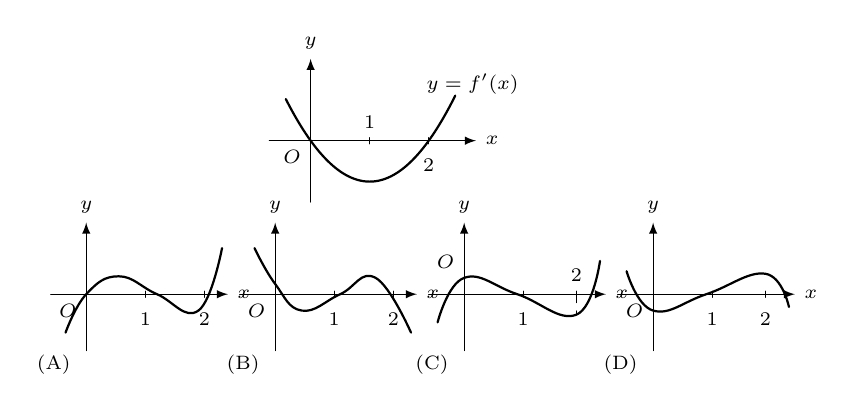
\begin{tikzpicture}[line cap=round,line join=round,>=latex,x=0.75cm,y=0.65cm,every node/.style={font=\scriptsize}]
  % Top: prompt curve y = f'(x)
  \begin{scope}[shift={(3.8,3.0)}]
    \draw[->] (-0.7,0) -- (2.8,0) node[right] {$x$};
    \draw[->] (0,-1.2) -- (0,1.6) node[above] {$y$};
    \node[below left] at (0,0) {$O$};
    \draw[thick,domain=-0.42:2.45,samples=80] plot (\x,{0.8*\x*(\x-2)});
    \draw (1,0.06) -- (1,-0.06) node[above=2pt] {$1$};
    \draw (2,0.06) -- (2,-0.06) node[below=2pt] {$2$};
    \node[right] at (1.8,1.1) {$y = f'(x)$};
  \end{scope}

  % Bottom: Four candidate graphs (A), (B), (C), (D)
  % (A)
  \begin{scope}[shift={(0,0)}]
    \draw[->] (-0.6,0) -- (2.4,0) node[right] {$x$};
    \draw[->] (0,-1.1) -- (0,1.4) node[above] {$y$};
    \node[below left] at (0,0) {$O$};
    \draw[thick] plot[smooth,tension=0.75] coordinates {(-0.35,-0.75) (0,0) (0.55,0.35) (1.2,0) (1.9,-0.32) (2.3,0.9)};
    \draw (1,0.06) -- (1,-0.06) node[below=2pt] {$1$};
    \draw (2,0.06) -- (2,-0.06) node[below=2pt] {$2$};
    \node[below left] at (-0.1,-1.0) {(A)};
  \end{scope}

  % (B)
  \begin{scope}[shift={(3.2,0)}]
    \draw[->] (-0.6,0) -- (2.4,0) node[right] {$x$};
    \draw[->] (0,-1.1) -- (0,1.4) node[above] {$y$};
    \node[below left] at (0,0) {$O$};
    \draw[thick] plot[smooth,tension=0.75] coordinates {(-0.35,0.9) (0,0.2) (0.45,-0.32) (1.1,0) (1.7,0.32) (2.3,-0.75)};
    \draw (1,0.06) -- (1,-0.06) node[below=2pt] {$1$};
    \draw (2,0.06) -- (2,-0.06) node[below=2pt] {$2$};
    \node[below left] at (-0.1,-1.0) {(B)};
  \end{scope}

  % (C) - Correct option
  \begin{scope}[shift={(6.4,0)}]
    \draw[->] (-0.6,0) -- (2.4,0) node[right] {$x$};
    \draw[->] (0,-1.1) -- (0,1.4) node[above] {$y$};
    \node[above left] at (0,0.32) {$O$};
    \draw[thick] plot[smooth,tension=0.75] coordinates {(-0.45,-0.55) (0,0.32) (0.9,0) (1.9,-0.4) (2.3,0.65)};
    \draw[dashed] (1.9,0) -- (1.9,-0.4);
    \draw (1,0.06) -- (1,-0.06) node[below=2pt] {$1$};
    \draw (1.9,0.06) -- (1.9,-0.06) node[above=2pt] {$2$};
    \node[below left] at (-0.1,-1.0) {(C)};
  \end{scope}

  % (D)
  \begin{scope}[shift={(9.6,0)}]
    \draw[->] (-0.6,0) -- (2.4,0) node[right] {$x$};
    \draw[->] (0,-1.1) -- (0,1.4) node[above] {$y$};
    \node[below left] at (0,0) {$O$};
    \draw[thick] plot[smooth,tension=0.75] coordinates {(-0.45,0.45) (0,-0.32) (0.9,0) (1.9,0.4) (2.3,-0.25)};
    \draw (1,0.06) -- (1,-0.06) node[below=2pt] {$1$};
    \draw (1.9,0.06) -- (1.9,-0.06) node[below=2pt] {$2$};
    \node[below left] at (-0.1,-1.0) {(D)};
  \end{scope}
\end{tikzpicture}
\end{center}
\nopagebreak[4]
观察导函数 $y = f'(x)$ 的图象特征：
1. 当 $x < 0$ 时，$f'(x) > 0$，函数 $f(x)$ 在 $(-\infty, 0)$ 上单调递增；
2. 当 $x = 0$ 时，$f'(0) = 0$，且两侧导数符号由正变负，因此 $x = 0$ 为函数 $f(x)$ 的极大值点；
3. 当 $0 < x < 2$ 时，$f'(x) < 0$，函数 $f(x)$ 在 $(0, 2)$ 上单调递减；在 $x = 1$ 处导函数取得极小值，说明原函数在 $x = 1$ 处的切线斜率负得最多，对应拐点；
4. 当 $x = 2$ 时，$f'(2) = 0$，且两侧导数符号由负变正，因此 $x = 2$ 为函数 $f(x)$ 的极小值点；
5. 当 $x > 2$ 时，$f'(x) > 0$，函数 $f(x)$ 在 $(2, +\infty)$ 上单调递增．

逐项对比四个选项的图象：
\begin{itemize}
\item 选项 A：在原点处单调递增，极大值点在区间 $(0, 1)$ 内，与 $f'(0) = 0$ 不符；
\item 选项 B：在原点处单调递减，$x = 0$ 处不是极大值点，不符；
\item 选项 C：在 $x < 0$ 上递增，极大值点恰好落在 $y$ 轴上（$x = 0$ 处取得峰值）；在 $(0, 2)$ 上递减，极小值点恰好在 $x = 2$ 处（对齐虚线谷值）；在 $x > 2$ 上递增，完全符合；
\item 选项 D：$x = 0$ 处为极小值点，$x = 2$ 处为极大值点，极值性质颠倒，不符．
\end{itemize}
综上，最有可能的图象是 C．
故选 C．

\gkanswer{答案：C}

\end{answer}
\begin{answer}
\gksolhead{12}{}

\textbf{题目}：

若 $f(x)$ 和 $g(x)$ 都是定义在实数集 $\mathbf{R}$ 上的函数，且方程 $x - f[g(x)] = 0$ 有实数解，则 $g[f(x)]$ 不可能是\mbox{（　　）}

\begin{gkopts}(2)
\task A．$x^2 + x - \dfrac{1}{5}$
\task B．$x^2 + x + \dfrac{1}{5}$
\task C．$x^2 - \dfrac{1}{5}$
\task D．$x^2 + \dfrac{1}{5}$
\end{gkopts}

\Needspace{4\baselineskip}
\textbf{解析}

由题意，方程 $x - f[g(x)] = 0$ 有实数解，设该实数解为 $x_0 \in \mathbf{R}$．
\Needspace{5\baselineskip}
则有
\nopagebreak[4]
\[
f[g(x_0)] = x_0.
\]
\Needspace{5\baselineskip}
在等式两边同时作用外层函数 $g$，得
\nopagebreak[4]
\[
g\big(f[g(x_0)]\big) = g(x_0).
\]
\Needspace{5\baselineskip}
令实数 $u_0 = g(x_0) \in \mathbf{R}$，则上式即为
\nopagebreak[4]
\[
g[f(u_0)] = u_0.
\]
这表明：方程 $g[f(x)] = x$ 必存在实数解 $x = u_0$（即复合函数 $y = g[f(x)]$ 必须存在不动点，其图象与直线 $y = x$ 必须有公共点）．
下面检验各个选项中方程 $g[f(x)] = x$ 是否存在实数解：
对于选项 A：
$x^2 + x - \dfrac{1}{5} = x \iff x^2 - \dfrac{1}{5} = 0 \iff x = \pm\dfrac{\sqrt{5}}{5}$，有实数解；
对于选项 B：
$x^2 + x + \dfrac{1}{5} = x \iff x^2 + \dfrac{1}{5} = 0$，因为对任意实数 $x$ 恒有 $x^2 \geqslant 0$，所以 $x^2 + \dfrac{1}{5} \geqslant \dfrac{1}{5} > 0$，方程无实数解！这与“$g[f(x)] = x$ 必有实数解”矛盾，故 $g[f(x)]$ 不可能是 $x^2 + x + \dfrac{1}{5}$；
对于选项 C：
$x^2 - \dfrac{1}{5} = x \iff x^2 - x - \dfrac{1}{5} = 0$，判别式 $\Delta = 1 + \dfrac{4}{5} = \dfrac{9}{5} > 0$，有两实数解；
对于选项 D：
$x^2 + \dfrac{1}{5} = x \iff x^2 - x + \dfrac{1}{5} = 0$，判别式 $\Delta = 1 - \dfrac{4}{5} = \dfrac{1}{5} > 0$，有两实数解．
综上，$g[f(x)]$ 不可能是选项 B．
故选 B．

\gkanswer{答案：B}

\end{answer}
\begin{answer}
\gksolhead{13}{}

\textbf{题目}：

已知 $f(x) = \begin{cases} 1, & x \geqslant 0, \\ -1, & x < 0, \end{cases}$ 则不等式 $x + (x + 2) \cdot f(x + 2) \leqslant 5$ 的解集是 \underline{\hspace{3cm}}．

\Needspace{4\baselineskip}
\textbf{解析}

已知分段函数 $f(x) = \begin{cases} 1, & x \geqslant 0, \\ -1, & x < 0. \end{cases}$
对于不等式 $x + (x + 2) \cdot f(x + 2) \leqslant 5$，分两种情况讨论自变量 $x + 2$ 的取值符号：

（1）当 $x + 2 \geqslant 0$，即 $x \geqslant -2$ 时：
\Needspace{5\baselineskip}
$f(x + 2) = 1$．不等式化为
\nopagebreak[4]
\[
x + (x + 2) \cdot 1 \leqslant 5 \implies 2x + 2 \leqslant 5 \implies 2x \leqslant 3 \implies x \leqslant \frac{3}{2}.
\]
结合前提条件 $x \geqslant -2$，得 $-2 \leqslant x \leqslant \dfrac{3}{2}$．

（2）当 $x + 2 < 0$，即 $x < -2$ 时：
\Needspace{5\baselineskip}
$f(x + 2) = -1$．不等式化为
\nopagebreak[4]
\[
x + (x + 2) \cdot (-1) \leqslant 5 \implies x - x - 2 \leqslant 5 \implies -2 \leqslant 5.
\]
此不等式对所有 $x < -2$ 恒成立，因此所有 $x < -2$ 均满足原不等式．

\Needspace{5\baselineskip}
综合上述两种情况，不等式的解集为
\nopagebreak[4]
\[
(-\infty, -2) \cup \left[-2, \frac{3}{2}\right] = \left(-\infty, \frac{3}{2}\right],
\]
即 $\left\{x \;\middle|\; x \leqslant \dfrac{3}{2}\right\}$．

\gkanswer{答案：$\left(-\infty, \dfrac{3}{2}\right]$（或 $\{x \mid x \leqslant \dfrac{3}{2}\}$）}

\end{answer}
\begin{answer}
\gksolhead{14}{}

\textbf{题目}：

已知平面上三点 $A$、$B$、$C$ 满足 $|\vec{AB}| = 3$，$|\vec{BC}| = 4$，$|\vec{CA}| = 5$，则 $\vec{AB} \cdot \vec{BC} + \vec{BC} \cdot \vec{CA} + \vec{CA} \cdot \vec{AB}$ 的值等于 \underline{\hspace{3cm}}．

\Needspace{4\baselineskip}
\textbf{解析}

\Needspace{5\baselineskip}
因为 $A, B, C$ 是平面上三点，所以首尾相连的向量之和为零向量：
\nopagebreak[4]
\[
\vec{AB} + \vec{BC} + \vec{CA} = \vec{0}.
\]
\Needspace{5\baselineskip}
在等式两边对自身作数量积（即求模平方）：
\nopagebreak[4]
\[
|\vec{AB} + \vec{BC} + \vec{CA}|^2 = 0.
\]
\Needspace{5\baselineskip}
展开左端得
\nopagebreak[4]
\[
|\vec{AB}|^2 + |\vec{BC}|^2 + |\vec{CA}|^2 + 2(\vec{AB} \cdot \vec{BC} + \vec{BC} \cdot \vec{CA} + \vec{CA} \cdot \vec{AB}) = 0.
\]
\Needspace{5\baselineskip}
代入已知线段长度 $|\vec{AB}| = 3$，$|\vec{BC}| = 4$，$|\vec{CA}| = 5$：
\nopagebreak[4]
\[
3^2 + 4^2 + 5^2 + 2(\vec{AB} \cdot \vec{BC} + \vec{BC} \cdot \vec{CA} + \vec{CA} \cdot \vec{AB}) = 0,
\]
\Needspace{5\baselineskip}
即
\nopagebreak[4]
\[
9 + 16 + 25 + 2(\vec{AB} \cdot \vec{BC} + \vec{BC} \cdot \vec{CA} + \vec{CA} \cdot \vec{AB}) = 0 \implies 50 + 2(\vec{AB} \cdot \vec{BC} + \vec{BC} \cdot \vec{CA} + \vec{CA} \cdot \vec{AB}) = 0.
\]
\Needspace{5\baselineskip}
解得
\nopagebreak[4]
\[
\vec{AB} \cdot \vec{BC} + \vec{BC} \cdot \vec{CA} + \vec{CA} \cdot \vec{AB} = -25.
\]

\gkanswer{答案：$-25$}

\end{answer}
\begin{answer}
\gksolhead{15}{}

\textbf{题目}：

设坐标平面内有一个质点从原点出发，沿 $x$ 轴跳动，每次向正方向或负方向跳 $1$ 个单位，经过 $5$ 次跳动质点落在点 $(3, 0)$（允许重复过此点）处，则质点不同的运动方法共有 \underline{\hspace{3cm}} 种．（用数字作答）

\Needspace{4\baselineskip}
\textbf{解析}

设质点在 5 次跳动中，向正方向跳动了 $a$ 次，向负方向跳动了 $b$ 次．
\Needspace{5\baselineskip}
因为总共跳动了 5 次，所以
\nopagebreak[4]
\[
a + b = 5.
\]
\Needspace{5\baselineskip}
质点从原点出发，每次跳动 1 个单位，经过 5 次跳动落在点 $(3, 0)$ 处，所以总位移为
\nopagebreak[4]
\[
a - b = 3.
\]
\Needspace{5\baselineskip}
联立上述两式，解得
\nopagebreak[4]
\[
a = 4, \quad b = 1.
\]
即质点必须在 5 次跳动中恰有 4 次向正方向跳动、1 次向负方向跳动．
\Needspace{5\baselineskip}
这相当于从 5 次跳动中选出 4 次向正方向跳动，不同的运动方法总数为组合数
\nopagebreak[4]
\[
\mathrm{C}_5^4 = 5.
\]
所以不同的运动方法共有 $5$ 种．

\gkanswer{答案：$5$}

\end{answer}
\begin{answer}
\gksolhead{16}{}

\textbf{题目}：

已知平面 $\alpha$ 和平面 $\beta$ 交于直线 $l$，$P$ 是空间一点，$PA \perp \alpha$，垂足为 $A$，$PB \perp \beta$，垂足为 $B$，且 $PA = 1$，$PB = 2$，若点 $A$ 在 $\beta$ 内的射影与点 $B$ 在 $\alpha$ 内的射影重合，则点 $P$ 到 $l$ 的距离为 \underline{\hspace{3cm}}．

\Needspace{4\baselineskip}
\textbf{解析}

设点 $A$ 在平面 $\beta$ 内的射影为点 $Q$．
由题意，点 $B$ 在平面 $\alpha$ 内的射影也与点 $Q$ 重合．
因为 $Q$ 是点 $A$ 在 $\beta$ 内的射影，所以 $AQ \perp \beta$；又已知 $PB \perp \beta$，所以 $AQ \parallel PB$．
因为 $Q$ 是点 $B$ 在 $\alpha$ 内的射影，所以 $BQ \perp \alpha$；又已知 $PA \perp \alpha$，所以 $BQ \parallel PA$．
因此在空间四边形 $PAQB$ 中，$PA \parallel BQ$ 且 $PB \parallel AQ$，故四边形 $PAQB$ 为平面平行四边形．
又因为 $PA \perp \alpha$，而交线 $l \subset \alpha$，所以 $PA \perp l$；
同理 $PB \perp \beta$，而交线 $l \subset \beta$，所以 $PB \perp l$．
因为 $PA \perp l$ 且 $PB \perp l$，$PA \cap PB = P$，所以直线 $l \perp$ 平面 $PAB$（即 $l$ 垂直于四边形 $PAQB$ 所在的整个平面）．
设直线 $l$ 与平面 $PAQB$ 相交于点 $O$．
因为 $l \perp$ 平面 $PAQB$，所以点 $P$ 到直线 $l$ 的距离即为线段 $PO$ 的长度．
再者，点 $Q$ 在平面 $\alpha$ 内（作为射影），且点 $Q$ 也在平面 $\beta$ 内（作为射影），所以点 $Q$ 落在交线 $l = \alpha \cap \beta$ 上．
而在平面 $PAQB$ 内，交线 $l$ 与该平面只有一个交点 $O$，因此点 $Q$ 必与点 $O$ 重合，即 $Q = O$．
在平面四边形 $PAOB$ 中：
因为 $PA \perp \alpha$，直线 $OA \subset \alpha$，所以 $PA \perp OA$，$\angle PAO = 90^\circ$；
因为 $PB \perp \beta$，直线 $OB \subset \beta$，所以 $PB \perp OB$，$\angle PBO = 90^\circ$．
又有 $PA \parallel OB$ 且 $PB \parallel OA$，所以四边形 $PAOB$ 为矩形．
在矩形 $PAOB$ 中，$OA = PB = 2$，$OB = PA = 1$．
\Needspace{5\baselineskip}
由勾股定理，对角线长度为
\nopagebreak[4]
\[
PO = \sqrt{PA^2 + OA^2} = \sqrt{1^2 + 2^2} = \sqrt{5}.
\]
所以点 $P$ 到直线 $l$ 的距离为 $\sqrt{5}$．

\gkanswer{答案：$\sqrt{5}$}

\end{answer}
\begin{answer}
\gksolhead{17}{}

\textbf{题目}：

（本小题满分 12 分）

在 $\triangle ABC$ 中，角 $A$、$B$、$C$ 所对的边分别为 $a$、$b$、$c$，且 $\cos A = \dfrac{1}{3}$．

（1）求 $\sin^2\dfrac{B+C}{2} + \cos 2A$ 的值；

（2）若 $a = \sqrt{3}$，求 $bc$ 的最大值．

\Needspace{4\baselineskip}
\textbf{解析}

（1）因为 $A, B, C$ 为 $\triangle ABC$ 的三个内角，所以 $A + B + C = \pi$，进而 $\dfrac{B+C}{2} = \dfrac{\pi}{2} - \dfrac{A}{2}$．
\Needspace{5\baselineskip}
由诱导公式与半角降幂公式，
\nopagebreak[4]
\[
\sin\frac{B+C}{2} = \sin\left(\frac{\pi}{2} - \frac{A}{2}\right) = \cos\frac{A}{2},
\]
\nopagebreak[4]
\[
\sin^2\frac{B+C}{2} = \cos^2\frac{A}{2} = \frac{1 + \cos A}{2}.
\]
\Needspace{5\baselineskip}
已知 $\cos A = \dfrac{1}{3}$，代入得
\nopagebreak[4]
\[
\sin^2\frac{B+C}{2} = \frac{1 + \dfrac{1}{3}}{2} = \frac{2}{3}.
\]
\Needspace{5\baselineskip}
又由二倍角余弦公式，
\nopagebreak[4]
\[
\cos 2A = 2\cos^2 A - 1 = 2\left(\frac{1}{3}\right)^2 - 1 = \frac{2}{9} - 1 = -\frac{7}{9}.
\]
\Needspace{5\baselineskip}
所以
\nopagebreak[4]
\[
\sin^2\frac{B+C}{2} + \cos 2A = \frac{2}{3} + \left(-\frac{7}{9}\right) = \frac{6}{9} - \frac{7}{9} = -\frac{1}{9}.
\]

\Needspace{5\baselineskip}
（2）在 $\triangle ABC$ 中，由余弦定理，
\nopagebreak[4]
\[
a^2 = b^2 + c^2 - 2bc\cos A.
\]
\Needspace{5\baselineskip}
已知 $a = \sqrt{3}$，$\cos A = \dfrac{1}{3}$，代入得
\nopagebreak[4]
\[
3 = b^2 + c^2 - \frac{2}{3}bc.
\]
\Needspace{5\baselineskip}
由基本不等式 $b^2 + c^2 \geqslant 2bc$（当且仅当 $b = c$ 时等号成立），得
\nopagebreak[4]
\[
3 \geqslant 2bc - \frac{2}{3}bc = \frac{4}{3}bc.
\]
\Needspace{5\baselineskip}
解得
\nopagebreak[4]
\[
bc \leqslant \frac{9}{4}.
\]
当且仅当 $b = c = \dfrac{3}{2}$ 时等号成立，此时三角形三边长为 $\dfrac{3}{2}, \dfrac{3}{2}, \sqrt{3}$，满足构成三角形的条件．
所以 $bc$ 的最大值为 $\dfrac{9}{4}$．

\gkanswer{答案：（1）$-\dfrac{1}{9}$；（2）$\dfrac{9}{4}$}

\end{answer}
\begin{answer}
\gksolhead{18}{}

\textbf{题目}：

（本小题满分 12 分）

盒子中有大小相同的球 10 个，其中标号为 1 的球 3 个，标号为 2 的球 4 个，标号为 5 的球 3 个，第一次从盒子中任取 1 个球，放回后第二次再任取 1 个球（假设取到每个球的可能性都相同）．记第一次与第二次取到球的标号之和为 $\xi$．

（1）求随机变量 $\xi$ 的分布列；

（2）求随机变量 $\xi$ 的期望 $\mathrm{E}\xi$．

\Needspace{4\baselineskip}
\textbf{解析}

从装有 10 个球的盒子中有放回地抽取 2 次，两次抽取相互独立．
\Needspace{5\baselineskip}
每次抽取取到各个标号球的概率分别为
\nopagebreak[4]
\[
P(X = 1) = \frac{3}{10}, \quad P(X = 2) = \frac{4}{10} = \frac{2}{5}, \quad P(X = 5) = \frac{3}{10}.
\]
记第一次抽到的球标号为 $X_1$，第二次抽到的球标号为 $X_2$，$X_1$ 与 $X_2$ 独立同分布．
随机变量 $\xi = X_1 + X_2$．

（1）随机变量 $\xi$ 的所有可能取值为 $2, 3, 4, 6, 7, 10$．
各可能取值的概率分别计算如下：
\begin{itemize}
\item $P(\xi = 2) = P(X_1 = 1, X_2 = 1) = \dfrac{3}{10} \times \dfrac{3}{10} = \dfrac{9}{100}$；
\item $P(\xi = 3) = P(X_1 = 1, X_2 = 2) + P(X_1 = 2, X_2 = 1) = 2 \times \left(\dfrac{3}{10} \times \dfrac{4}{10}\right) = \dfrac{24}{100} = \dfrac{6}{25}$；
\item $P(\xi = 4) = P(X_1 = 2, X_2 = 2) = \dfrac{4}{10} \times \dfrac{4}{10} = \dfrac{16}{100} = \dfrac{4}{25}$；
\item $P(\xi = 6) = P(X_1 = 1, X_2 = 5) + P(X_1 = 5, X_2 = 1) = 2 \times \left(\dfrac{3}{10} \times \dfrac{3}{10}\right) = \dfrac{18}{100} = \dfrac{9}{50}$；
\item $P(\xi = 7) = P(X_1 = 2, X_2 = 5) + P(X_1 = 5, X_2 = 2) = 2 \times \left(\dfrac{4}{10} \times \dfrac{3}{10}\right) = \dfrac{24}{100} = \dfrac{6}{25}$；
\item $P(\xi = 10) = P(X_1 = 5, X_2 = 5) = \dfrac{3}{10} \times \dfrac{3}{10} = \dfrac{9}{100}$．
\end{itemize}

\Needspace{5\baselineskip}
检验全概率之和：
\nopagebreak[4]
\[
\frac{9}{100} + \frac{24}{100} + \frac{16}{100} + \frac{18}{100} + \frac{24}{100} + \frac{9}{100} = \frac{100}{100} = 1.
\]
因此随机变量 $\xi$ 的分布列为：

\begin{center}
\begin{tabular}{ccccccc}
\toprule
$\xi$ & 2 & 3 & 4 & 6 & 7 & 10 \\
\midrule
$P$ & $\dfrac{9}{100}$ & $\dfrac{6}{25}$ & $\dfrac{4}{25}$ & $\dfrac{9}{50}$ & $\dfrac{6}{25}$ & $\dfrac{9}{100}$ \\
\bottomrule
\end{tabular}
\end{center}

（2）求随机变量 $\xi$ 的数学期望：
\Needspace{5\baselineskip}
单次抽取的随机变量 $X_1$ 的数学期望为
\nopagebreak[4]
\[
\mathrm{E}X_1 = 1 \times \frac{3}{10} + 2 \times \frac{4}{10} + 5 \times \frac{3}{10} = \frac{3 + 8 + 15}{10} = \frac{26}{10} = 2.6.
\]
\Needspace{5\baselineskip}
由数学期望的线性性质，
\nopagebreak[4]
\[
\mathrm{E}\xi = \mathrm{E}(X_1 + X_2) = \mathrm{E}X_1 + \mathrm{E}X_2 = 2.6 + 2.6 = 5.2.
\]
（亦可由定义式直接计算：$\mathrm{E}\xi = 2 \times \dfrac{9}{100} + 3 \times \dfrac{24}{100} + 4 \times \dfrac{16}{100} + 6 \times \dfrac{18}{100} + 7 \times \dfrac{24}{100} + 10 \times \dfrac{9}{100} = \dfrac{18 + 72 + 64 + 108 + 168 + 90}{100} = \dfrac{520}{100} = 5.2$）．

\gkanswer{答案：（1）分布列见解析；（2）$5.2$（或 $\dfrac{26}{5}$）}

\end{answer}
\begin{answer}
\gksolhead{19}{}

\textbf{题目}：

（本小题满分 12 分）

如图，已知正方形 $ABCD$ 和矩形 $ACEF$ 所在的平面互相垂直，$AB = \sqrt{2}$，$AF = 1$，$M$ 是线段 $EF$ 的中点．

（1）求证：$AM \parallel$ 平面 $BDE$；

（2）求二面角 $A - DF - B$ 的大小．
\nopagebreak[4]
\begin{center}% Candidate source: src-e83c48821eaac4546df1607aa7bd47f8c49362fe9d091f3ff8accf356722e61c
% Source PDF SHA-256: 0a787b530b939cb104a802de2c27119b5d150bac7c4f0e78b069bc103f381232
% PDF page 1 (printed page 206), question 19.
% Redraw follows visible/hidden edges: square ABCD and rectangle ACEF perpendicular, point M midpoint of EF.
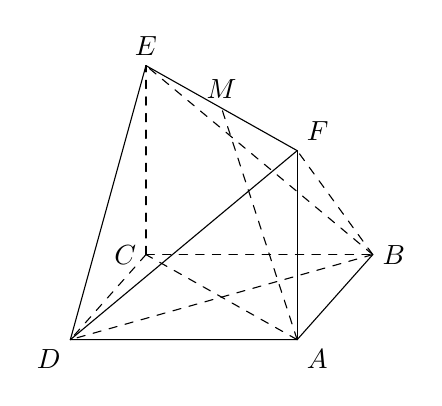
\begin{tikzpicture}[line cap=round,line join=round,>=latex,scale=1.2]
  % Vertex coordinates
  \coordinate (D) at (0,0);
  \coordinate (A) at (2.4,0);
  \coordinate (B) at (3.2,0.9);
  \coordinate (C) at (0.8,0.9);
  \coordinate (F) at (2.4,2.0);
  \coordinate (E) at (0.8,2.9);
  \coordinate (M) at (1.6,2.45);

  % Hidden (dashed) edges
  \draw[dashed] (C) -- (D);
  \draw[dashed] (C) -- (B);
  \draw[dashed] (C) -- (E);
  \draw[dashed] (A) -- (C);
  \draw[dashed] (B) -- (D);
  \draw[dashed] (B) -- (E);
  \draw[dashed] (B) -- (F);
  \draw[dashed] (A) -- (M);

  % Visible (solid) edges
  \draw (D) -- (A) -- (B);
  \draw (A) -- (F);
  \draw (D) -- (E);
  \draw (D) -- (F);
  \draw (E) -- (F);

  % Vertex labels
  \node[below left] at (D) {$D$};
  \node[below right] at (A) {$A$};
  \node[right] at (B) {$B$};
  \node[left] at (C) {$C$};
  \node[above] at (E) {$E$};
  \node[above right] at (F) {$F$};
  \node[above] at (M) {$M$};
\end{tikzpicture}
\end{center}
\nopagebreak[4]
\Needspace{4\baselineskip}
\textbf{解析}
\nopagebreak[4]
\begin{center}% Candidate source: src-e83c48821eaac4546df1607aa7bd47f8c49362fe9d091f3ff8accf356722e61c
% Source PDF SHA-256: 0a787b530b939cb104a802de2c27119b5d150bac7c4f0e78b069bc103f381232
% PDF page 1 (printed page 206), question 19.
% Redraw follows visible/hidden edges: square ABCD and rectangle ACEF perpendicular, point M midpoint of EF.
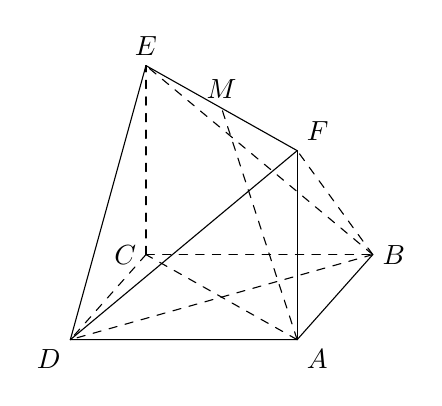
\begin{tikzpicture}[line cap=round,line join=round,>=latex,scale=1.2]
  % Vertex coordinates
  \coordinate (D) at (0,0);
  \coordinate (A) at (2.4,0);
  \coordinate (B) at (3.2,0.9);
  \coordinate (C) at (0.8,0.9);
  \coordinate (F) at (2.4,2.0);
  \coordinate (E) at (0.8,2.9);
  \coordinate (M) at (1.6,2.45);

  % Hidden (dashed) edges
  \draw[dashed] (C) -- (D);
  \draw[dashed] (C) -- (B);
  \draw[dashed] (C) -- (E);
  \draw[dashed] (A) -- (C);
  \draw[dashed] (B) -- (D);
  \draw[dashed] (B) -- (E);
  \draw[dashed] (B) -- (F);
  \draw[dashed] (A) -- (M);

  % Visible (solid) edges
  \draw (D) -- (A) -- (B);
  \draw (A) -- (F);
  \draw (D) -- (E);
  \draw (D) -- (F);
  \draw (E) -- (F);

  % Vertex labels
  \node[below left] at (D) {$D$};
  \node[below right] at (A) {$A$};
  \node[right] at (B) {$B$};
  \node[left] at (C) {$C$};
  \node[above] at (E) {$E$};
  \node[above right] at (F) {$F$};
  \node[above] at (M) {$M$};
\end{tikzpicture}
\end{center}
\nopagebreak[4]
（1）证明：
设正方形 $ABCD$ 的对角线 $AC$ 与 $BD$ 相交于点 $O$，连接 $OE$．
在正方形 $ABCD$ 中，点 $O$ 是线段 $AC$ 的中点，且 $OA = \dfrac{1}{2}AC$．
在矩形 $ACEF$ 中，$EF \parallel AC$ 且 $EF = AC$．
\Needspace{5\baselineskip}
已知点 $M$ 是线段 $EF$ 的中点，所以
\nopagebreak[4]
\[
EM \parallel AC, \quad EM = \frac{1}{2}EF = \frac{1}{2}AC.
\]
因此 $EM \parallel OA$ 且 $EM = OA$．
\Needspace{5\baselineskip}
从而四边形 $AOEM$ 为平行四边形，所以
\nopagebreak[4]
\[
AM \parallel OE.
\]
因为 $OE \subset$ 平面 $BDE$，且直线 $AM \not\subset$ 平面 $BDE$，
所以 $AM \parallel$ 平面 $BDE$．

（2）解：
在正方形 $ABCD$ 中，$AB = \sqrt{2}$，所以 $AD = \sqrt{2}$，$AC = BD = \sqrt{(\sqrt{2})^2 + (\sqrt{2})^2} = 2$．
对角线交点 $O$ 满足 $OA = OB = OC = OD = 1$，且 $AC \perp BD$．
已知矩形 $ACEF$ 所在的平面与正方形 $ABCD$ 所在的平面互相垂直，交线为 $AC$．
在矩形 $ACEF$ 中，$AF \perp AC$ 且 $AF = 1$．
因为平面 $ACEF \perp$ 平面 $ABCD$，$AF \subset$ 平面 $ACEF$，且 $AF \perp AC$，
所以 $AF \perp$ 平面 $ABCD$．
在三棱锥 $F - ABD$ 中：
底面 $\triangle ABD$ 是以 $\angle BAD = 90^\circ$ 的等腰直角三角形，$AB = AD = \sqrt{2}$，$BD = 2$．
$AF \perp$ 底面 $ABD$，高 $AF = 1$．
\Needspace{5\baselineskip}
在 Rt$\triangle FAD$ 中，$\angle FAD = 90^\circ$，$FA = 1$，$AD = \sqrt{2}$，由勾股定理得
\nopagebreak[4]
\[
FD = \sqrt{FA^2 + AD^2} = \sqrt{1^2 + (\sqrt{2})^2} = \sqrt{3}.
\]
\Needspace{5\baselineskip}
过点 $A$ 在平面 $ADF$ 内作 $AH \perp DF$ 于点 $H$，则
\nopagebreak[4]
\[
AH = \frac{AF \cdot AD}{FD} = \frac{1 \times \sqrt{2}}{\sqrt{3}} = \frac{\sqrt{6}}{3}.
\]
\Needspace{5\baselineskip}
因为 $AB \perp AD$ 且 $AB \perp AF$，$AD \cap AF = A$，所以
\nopagebreak[4]
\[
AB \perp \text{平面} FAD.
\]
\Needspace{5\baselineskip}
而直线 $DF \subset$ 平面 $FAD$，所以
\nopagebreak[4]
\[
AB \perp DF.
\]
\Needspace{5\baselineskip}
又因为 $AH \perp DF$ 且 $AB \perp DF$，$AH \cap AB = A$，所以
\nopagebreak[4]
\[
DF \perp \text{平面} ABH.
\]
\Needspace{5\baselineskip}
连接 $BH$，因为 $BH \subset$ 平面 $ABH$，所以
\nopagebreak[4]
\[
DF \perp BH.
\]
因此，$\angle AHB$ 为二面角 $A - DF - B$ 的平面角．
\Needspace{5\baselineskip}
又因为 $AB \perp$ 平面 $FAD$，且 $AH \subset$ 平面 $FAD$，所以
\nopagebreak[4]
\[
AB \perp AH, \quad \text{\text{即} } \angle HAB = 90^\circ.
\]
\Needspace{5\baselineskip}
所以在 Rt$\triangle HAB$ 中，
\nopagebreak[4]
\[
\tan\angle AHB = \frac{AB}{AH} = \frac{\sqrt{2}}{\dfrac{\sqrt{6}}{3}} = \frac{3\sqrt{2}}{\sqrt{6}} = \sqrt{3}.
\]
\Needspace{5\baselineskip}
因为 $\angle AHB \in (0, 180^\circ)$，所以
\nopagebreak[4]
\[
\angle AHB = 60^\circ.
\]
即二面角 $A - DF - B$ 的大小为 $60^\circ$（或 $\dfrac{\pi}{3}$）．

\gkanswer{答案：（1）证明见解析；（2）$60^\circ$（或 $\dfrac{\pi}{3}$）}

\end{answer}
\begin{answer}
\gksolhead{20}{}

\textbf{题目}：

（本小题满分 12 分）

设曲线 $y = \mathrm{e}^{-x}$（$x \geqslant 0$）在点 $M(t, \mathrm{e}^{-t})$ 处的切线 $l$ 与 $x$ 轴、$y$ 轴所围成的三角形面积为 $S(t)$．

（1）求切线 $l$ 的方程；

（2）求 $S(t)$ 的最大值．

\Needspace{4\baselineskip}
\textbf{解析}

\Needspace{5\baselineskip}
（1）对于曲线 $y = \mathrm{e}^{-x}$（$x \geqslant 0$），求导得
\nopagebreak[4]
\[
y' = -\mathrm{e}^{-x}.
\]
\Needspace{5\baselineskip}
在点 $M(t, \mathrm{e}^{-t})$ 处，切线 $l$ 的斜率为
\nopagebreak[4]
\[
k = -\mathrm{e}^{-t}.
\]
\Needspace{5\baselineskip}
所以切线 $l$ 的点斜式方程为
\nopagebreak[4]
\[
y - \mathrm{e}^{-t} = -\mathrm{e}^{-t}(x - t),
\]
\Needspace{5\baselineskip}
整理得斜截式方程
\nopagebreak[4]
\[
y = -\mathrm{e}^{-t}x + (t + 1)\mathrm{e}^{-t},
\]
\Needspace{5\baselineskip}
或一般式方程
\nopagebreak[4]
\[
x + \mathrm{e}^t y - t - 1 = 0.
\]

（2）求切线 $l$ 与两坐标轴的交点：
\Needspace{5\baselineskip}
令 $y = 0$，得切线与 $x$ 轴的交点横坐标为
\nopagebreak[4]
\[
x_0 = t + 1;
\]
\Needspace{5\baselineskip}
令 $x = 0$，得切线与 $y$ 轴的交点纵坐标为
\nopagebreak[4]
\[
y_0 = (t + 1)\mathrm{e}^{-t}.
\]
因为 $t \geqslant 0$，所以 $x_0 = t + 1 > 0$，$y_0 = (t + 1)\mathrm{e}^{-t} > 0$．
\Needspace{5\baselineskip}
切线 $l$ 与 $x$ 轴、$y$ 轴围成的直角三角形面积为
\nopagebreak[4]
\[
S(t) = \frac{1}{2} x_0 y_0 = \frac{1}{2}(t + 1)^2 \mathrm{e}^{-t}, \quad (t \geqslant 0).
\]
\Needspace{5\baselineskip}
对 $S(t)$ 关于 $t$ 求导：
\nopagebreak[4]
\[
S'(t) = \frac{1}{2} \left[ 2(t + 1)\mathrm{e}^{-t} - (t + 1)^2 \mathrm{e}^{-t} \right] = \frac{1}{2}(t + 1)[2 - (t + 1)]\mathrm{e}^{-t} = \frac{1}{2}(t + 1)(1 - t)\mathrm{e}^{-t}.
\]
因为 $t \geqslant 0$，所以 $\dfrac{1}{2}(t + 1)\mathrm{e}^{-t} > 0$：
\begin{itemize}
\item 当 $0 \leqslant t < 1$ 时，$1 - t > 0$，所以 $S'(t) > 0$，$S(t)$ 单调递增；
\item 当 $t > 1$ 时，$1 - t < 0$，所以 $S'(t) < 0$，$S(t)$ 单调递减．
\end{itemize}
\Needspace{5\baselineskip}
因此，当 $t = 1$ 时，$S(t)$ 取得极大值，也是在区间 $[0, +\infty)$ 上的最大值：
\nopagebreak[4]
\[
S(1) = \frac{1}{2}(1 + 1)^2 \mathrm{e}^{-1} = \frac{2}{\mathrm{e}}.
\]
端点处 $S(0) = \dfrac{1}{2} < \dfrac{2}{\mathrm{e}}$．
所以 $S(t)$ 的最大值为 $\dfrac{2}{\mathrm{e}}$．

\gkanswer{答案：（1）$y = -\mathrm{e}^{-t}x + (t+1)\mathrm{e}^{-t}$（或 $x + \mathrm{e}^t y - t - 1 = 0$）；（2）$\dfrac{2}{\mathrm{e}}$}

\end{answer}
\begin{answer}
\gksolhead{21}{}

\textbf{题目}：

（本小题满分 12 分）

已知双曲线的中心在原点，右顶点为 $A(1, 0)$，点 $P$、$Q$ 在双曲线的右支上，点 $M(m, 0)$ 到直线 $AP$ 的距离为 $1$．

（1）若直线 $AP$ 的斜率为 $k$，且 $|k| \in \left[\dfrac{\sqrt{3}}{3}, \sqrt{3}\right]$，求实数 $m$ 的取值范围；

（2）当 $m = \sqrt{2} + 1$ 时，$\triangle APQ$ 的内心恰好是点 $M$，求此双曲线的方程．

\Needspace{4\baselineskip}
\textbf{解析}

（1）双曲线的中心在原点，右顶点为 $A(1, 0)$．
\Needspace{5\baselineskip}
直线 $AP$ 经过点 $A(1, 0)$，斜率为 $k$，其方程为
\nopagebreak[4]
\[
y - 0 = k(x - 1) \implies kx - y - k = 0.
\]
\Needspace{5\baselineskip}
点 $M(m, 0)$ 到直线 $AP$ 的距离为 $1$．由点到直线距离公式，
\nopagebreak[4]
\[
d = \frac{|k m - 0 - k|}{\sqrt{k^2 + (-1)^2}} = \frac{|k(m - 1)|}{\sqrt{k^2 + 1}} = 1.
\]
\Needspace{5\baselineskip}
两边平方得
\nopagebreak[4]
\[
k^2(m - 1)^2 = k^2 + 1 \implies (m - 1)^2 = 1 + \frac{1}{k^2}.
\]
\Needspace{5\baselineskip}
因为 $|k| \in \left[\dfrac{\sqrt{3}}{3}, \sqrt{3}\right]$，所以 $k^2 \in \left[\dfrac{1}{3}, 3\right]$，进而
\nopagebreak[4]
\[
\frac{1}{k^2} \in \left[\frac{1}{3}, 3\right].
\]
\Needspace{5\baselineskip}
因此
\nopagebreak[4]
\[
(m - 1)^2 = 1 + \frac{1}{k^2} \in \left[1 + \frac{1}{3}, 1 + 3\right] = \left[\frac{4}{3}, 4\right].
\]
\Needspace{5\baselineskip}
开平方得
\nopagebreak[4]
\[
\frac{2\sqrt{3}}{3} \leqslant |m - 1| \leqslant 2.
\]
解此绝对值不等式：
\begin{itemize}
\item 若 $m - 1 \geqslant 0$，则 $\dfrac{2\sqrt{3}}{3} \leqslant m - 1 \leqslant 2 \implies 1 + \dfrac{2\sqrt{3}}{3} \leqslant m \leqslant 3$；
\item 若 $m - 1 \leqslant 0$，则 $-2 \leqslant m - 1 \leqslant -\dfrac{2\sqrt{3}}{3} \implies -1 \leqslant m \leqslant 1 - \dfrac{2\sqrt{3}}{3}$．
\end{itemize}
综上，实数 $m$ 的取值范围为 $\left[-1, 1 - \dfrac{2\sqrt{3}}{3}\right] \cup \left[1 + \dfrac{2\sqrt{3}}{3}, 3\right]$．

（2）当 $m = \sqrt{2} + 1$ 时，点 $M(\sqrt{2} + 1, 0)$．
因为 $\triangle APQ$ 的内心恰好是点 $M$，所以点 $M$ 到三边 $AP$、$AQ$、$PQ$ 的距离均相等，且射线 $AM$ 平分 $\angle PAQ$．
已知顶点 $A(1, 0)$ 与内心 $M(\sqrt{2} + 1, 0)$ 均在 $x$ 轴上，且 $m > 1$，所以射线 $AM$ 即为 $x$ 轴正半轴．
因此，$x$ 轴平分 $\angle PAQ$．
由对称性，直线 $AP$ 与直线 $AQ$ 关于 $x$ 轴对称．
设直线 $AP$ 的斜率为 $k$（不妨设 $k > 0$），则直线 $AQ$ 的斜率为 $-k$．
\Needspace{5\baselineskip}
由（1）中的距离关系，当 $m = \sqrt{2} + 1$ 时，
\nopagebreak[4]
\[
(\sqrt{2} + 1 - 1)^2 = 1 + \frac{1}{k^2} \implies 2 = 1 + \frac{1}{k^2} \implies \frac{1}{k^2} = 1 \implies k^2 = 1.
\]
因为 $k > 0$，所以 $k = 1$．
因此直线 $AP$ 的方程为 $y = x - 1$，直线 $AQ$ 的方程为 $y = -(x - 1)$．
因为双曲线关于 $x$ 轴对称，而直线 $AP$ 与 $AQ$ 关于 $x$ 轴对称，所以它们与双曲线右支的交点 $P$ 与 $Q$ 也关于 $x$ 轴对称．
因此，线段 $PQ$ 垂直于 $x$ 轴，直线 $PQ$ 的方程为 $x = x_P$．
又因为 $M$ 是 $\triangle APQ$ 的内心，内切圆半径为 $r = 1$（点 $M$ 到直线 $AP$ 的距离），
所以点 $M$ 到直线 $PQ$ 的距离也等于 $1$．
因为内心 $M$ 位于 $\triangle APQ$ 内部，且 $A(1, 0)$ 在 $M$ 的左侧，所以点 $P$、$Q$ 的横坐标必大于点 $M$ 的横坐标，即 $x_P > m$．
\Needspace{5\baselineskip}
因此
\nopagebreak[4]
\[
x_P - m = 1 \implies x_P = m + 1 = \sqrt{2} + 2.
\]
\Needspace{5\baselineskip}
因为点 $P$ 在直线 $AP$（$y = x - 1$）上，所以
\nopagebreak[4]
\[
y_P = x_P - 1 = (\sqrt{2} + 2) - 1 = \sqrt{2} + 1.
\]
即点 $P$ 的坐标为 $(\sqrt{2} + 2, \sqrt{2} + 1)$．
\Needspace{5\baselineskip}
设双曲线的方程为
\nopagebreak[4]
\[
x^2 - \frac{y^2}{b^2} = 1 \quad (b > 0).
\]
\Needspace{5\baselineskip}
将点 $P(\sqrt{2} + 2, \sqrt{2} + 1)$ 的坐标代入双曲线方程：
\nopagebreak[4]
\[
(\sqrt{2} + 2)^2 - \frac{(\sqrt{2} + 1)^2}{b^2} = 1.
\]
\Needspace{5\baselineskip}
展开计算：
\nopagebreak[4]
\[
(\sqrt{2} + 2)^2 = 2 + 4\sqrt{2} + 4 = 6 + 4\sqrt{2},
\]
\nopagebreak[4]
\[
(\sqrt{2} + 1)^2 = 2 + 2\sqrt{2} + 1 = 3 + 2\sqrt{2}.
\]
\Needspace{5\baselineskip}
代入得
\nopagebreak[4]
\[
6 + 4\sqrt{2} - \frac{3 + 2\sqrt{2}}{b^2} = 1 \implies \frac{3 + 2\sqrt{2}}{b^2} = 5 + 4\sqrt{2}.
\]
\Needspace{5\baselineskip}
解得
\nopagebreak[4]
\[
b^2 = \frac{3 + 2\sqrt{2}}{5 + 4\sqrt{2}} = \frac{(3 + 2\sqrt{2})(5 - 4\sqrt{2})}{(5 + 4\sqrt{2})(5 - 4\sqrt{2})} = \frac{15 - 12\sqrt{2} + 10\sqrt{2} - 16}{25 - 32} = \frac{-1 - 2\sqrt{2}}{-7} = \frac{2\sqrt{2} + 1}{7}.
\]
\Needspace{5\baselineskip}
对 $b^2$ 进行有理化变形：
\nopagebreak[4]
\[
\frac{1}{b^2} = \frac{7}{2\sqrt{2} + 1} = \frac{7(2\sqrt{2} - 1)}{(2\sqrt{2} + 1)(2\sqrt{2} - 1)} = \frac{7(2\sqrt{2} - 1)}{8 - 1} = 2\sqrt{2} - 1.
\]
\Needspace{5\baselineskip}
所以双曲线的标准方程为
\nopagebreak[4]
\[
x^2 - (2\sqrt{2} - 1)y^2 = 1 \quad \left(\text{\text{或} } x^2 - \frac{y^2}{\dfrac{2\sqrt{2} + 1}{7}} = 1\right).
\]

\gkanswer{答案：（1）$\left[-1, 1 - \dfrac{2\sqrt{3}}{3}\right] \cup \left[1 + \dfrac{2\sqrt{3}}{3}, 3\right]$；（2）$x^2 - (2\sqrt{2}-1)y^2 = 1$（或 $x^2 - \dfrac{y^2}{\dfrac{2\sqrt{2}+1}{7}} = 1$）}

\end{answer}
\begin{answer}
\gksolhead{22}{}

\textbf{题目}：

（本小题满分 14 分）

如图，$\triangle OBC$ 的三个顶点坐标分别为 $(0, 0)$、$(1, 0)$、$(0, 2)$，设 $P_1$ 为线段 $BC$ 的中点，$P_2$ 为线段 $CO$ 的中点，$P_3$ 为线段 $OP_1$ 的中点，对于每一个正整数 $n$，$P_{n+3}$ 为线段 $P_n P_{n+1}$ 的中点，令 $P_n$ 的坐标为 $(x_n, y_n)$，$a_n = \dfrac{1}{2}y_n + y_{n+1} + y_{n+2}$．

（1）求 $a_1, a_2, a_3$ 及 $a_n$；

（2）证明 $y_{n+4} = 1 - \dfrac{y_n}{4}, n \in \mathbf{N}^*$；

（3）若记 $b_n = y_{4n+4} - y_{4n}, n \in \mathbf{N}^*$，证明 $\{b_n\}$ 是等比数列．
\nopagebreak[4]
\begin{center}% Candidate source: src-e83c48821eaac4546df1607aa7bd47f8c49362fe9d091f3ff8accf356722e61c
% Source PDF SHA-256: 0a787b530b939cb104a802de2c27119b5d150bac7c4f0e78b069bc103f381232
% PDF page 2 (printed page 207), question 22.
% Redraw follows visible relations: triangle OBC with recursive midpoint sequence P1, P2, P3, P4, P5.
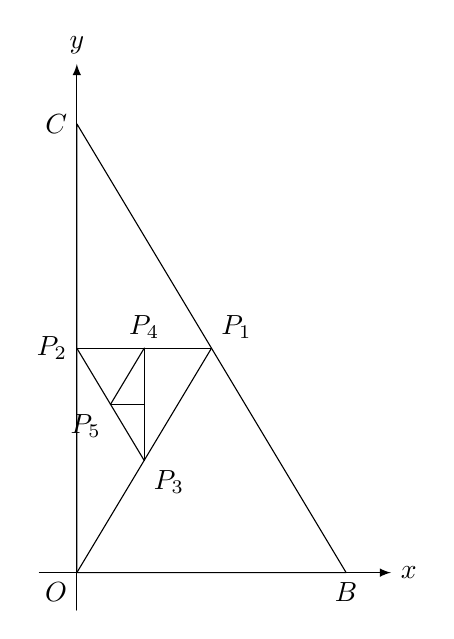
\begin{tikzpicture}[line cap=round,line join=round,>=latex,scale=0.95]
  % Coordinates for triangle OBC
  \coordinate (O) at (0,0);
  \coordinate (B) at (3.6,0);
  \coordinate (C) at (0,6.0);

  % Coordinates for midpoints P1 to P6
  \coordinate (P1) at (1.8,3.0);
  \coordinate (P2) at (0,3.0);
  \coordinate (P3) at (0.9,1.5);
  \coordinate (P4) at (0.9,3.0);
  \coordinate (P5) at (0.45,2.25);
  \coordinate (P6) at (0.9,2.25);

  % Axes
  \draw[->] (-0.5,0) -- (4.2,0) node[right] {$x$};
  \draw[->] (0,-0.5) -- (0,6.8) node[above] {$y$};

  % Triangle OBC
  \draw (C) -- (B) -- (O) -- cycle;

  % Spiral midpoint segments
  \draw (O) -- (P1);
  \draw (P1) -- (P2);
  \draw (P2) -- (P3);
  \draw (P3) -- (P4);
  \draw (P4) -- (P5);
  \draw (P5) -- (P6);

  % Labels
  \node[below left] at (O) {$O$};
  \node[below] at (B) {$B$};
  \node[left] at (C) {$C$};
  \node[above right] at (P1) {$P_1$};
  \node[left] at (P2) {$P_2$};
  \node[below right] at (P3) {$P_3$};
  \node[above] at (P4) {$P_4$};
  \node[below left] at (P5) {$P_5$};
\end{tikzpicture}
\end{center}
\nopagebreak[4]
\Needspace{4\baselineskip}
\textbf{解析}
\nopagebreak[4]
\begin{center}% Candidate source: src-e83c48821eaac4546df1607aa7bd47f8c49362fe9d091f3ff8accf356722e61c
% Source PDF SHA-256: 0a787b530b939cb104a802de2c27119b5d150bac7c4f0e78b069bc103f381232
% PDF page 2 (printed page 207), question 22.
% Redraw follows visible relations: triangle OBC with recursive midpoint sequence P1, P2, P3, P4, P5.
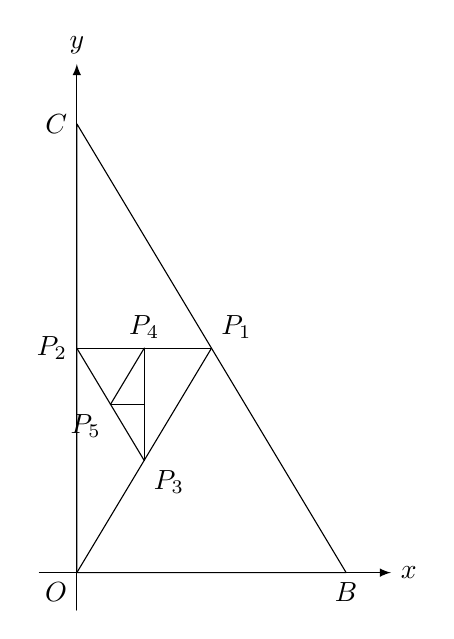
\begin{tikzpicture}[line cap=round,line join=round,>=latex,scale=0.95]
  % Coordinates for triangle OBC
  \coordinate (O) at (0,0);
  \coordinate (B) at (3.6,0);
  \coordinate (C) at (0,6.0);

  % Coordinates for midpoints P1 to P6
  \coordinate (P1) at (1.8,3.0);
  \coordinate (P2) at (0,3.0);
  \coordinate (P3) at (0.9,1.5);
  \coordinate (P4) at (0.9,3.0);
  \coordinate (P5) at (0.45,2.25);
  \coordinate (P6) at (0.9,2.25);

  % Axes
  \draw[->] (-0.5,0) -- (4.2,0) node[right] {$x$};
  \draw[->] (0,-0.5) -- (0,6.8) node[above] {$y$};

  % Triangle OBC
  \draw (C) -- (B) -- (O) -- cycle;

  % Spiral midpoint segments
  \draw (O) -- (P1);
  \draw (P1) -- (P2);
  \draw (P2) -- (P3);
  \draw (P3) -- (P4);
  \draw (P4) -- (P5);
  \draw (P5) -- (P6);

  % Labels
  \node[below left] at (O) {$O$};
  \node[below] at (B) {$B$};
  \node[left] at (C) {$C$};
  \node[above right] at (P1) {$P_1$};
  \node[left] at (P2) {$P_2$};
  \node[below right] at (P3) {$P_3$};
  \node[above] at (P4) {$P_4$};
  \node[below left] at (P5) {$P_5$};
\end{tikzpicture}
\end{center}
\nopagebreak[4]
由已知条件，$\triangle OBC$ 的三个顶点坐标分别为 $O(0, 0)$、$B(1, 0)$、$C(0, 2)$．
\begin{itemize}
\item 点 $P_1$ 为线段 $BC$ 的中点，由中点坐标公式：
\end{itemize}
\nopagebreak[4]
\[
x_1 = \frac{1 + 0}{2} = \frac{1}{2}, \quad y_1 = \frac{0 + 2}{2} = 1;
\]
\begin{itemize}
\item 点 $P_2$ 为线段 $CO$ 的中点：
\end{itemize}
\nopagebreak[4]
\[
x_2 = \frac{0 + 0}{2} = 0, \quad y_2 = \frac{2 + 0}{2} = 1;
\]
\begin{itemize}
\item 点 $P_3$ 为线段 $OP_1$ 的中点：
\end{itemize}
\nopagebreak[4]
\[
x_3 = \frac{0 + \dfrac{1}{2}}{2} = \frac{1}{4}, \quad y_3 = \frac{0 + 1}{2} = \frac{1}{2}.
\]
\Needspace{5\baselineskip}
对于每一个正整数 $n$，$P_{n+3}$ 为线段 $P_n P_{n+1}$ 的中点，因此纵坐标满足递推关系：
\nopagebreak[4]
\[
y_{n+3} = \frac{y_n + y_{n+1}}{2}, \quad n \in \mathbf{N}^*.
\]
\Needspace{5\baselineskip}
数列 $\{a_n\}$ 的定义为
\nopagebreak[4]
\[
a_n = \frac{1}{2}y_n + y_{n+1} + y_{n+2}.
\]

\Needspace{5\baselineskip}
（1）由递推关系，依次计算 $y_4, y_5$：
\nopagebreak[4]
\[
y_4 = \frac{y_1 + y_2}{2} = \frac{1 + 1}{2} = 1,
\]
\nopagebreak[4]
\[
y_5 = \frac{y_2 + y_3}{2} = \frac{1 + \dfrac{1}{2}}{2} = \frac{3}{4}.
\]
\Needspace{5\baselineskip}
代入数列定义计算各项：
\nopagebreak[4]
\[
a_1 = \frac{1}{2}y_1 + y_2 + y_3 = \frac{1}{2} \times 1 + 1 + \frac{1}{2} = 2,
\]
\nopagebreak[4]
\[
a_2 = \frac{1}{2}y_2 + y_3 + y_4 = \frac{1}{2} \times 1 + \frac{1}{2} + 1 = 2,
\]
\nopagebreak[4]
\[
a_3 = \frac{1}{2}y_3 + y_4 + y_5 = \frac{1}{2} \times \frac{1}{2} + 1 + \frac{3}{4} = \frac{1}{4} + 1 + \frac{3}{4} = 2.
\]
\Needspace{5\baselineskip}
考察相邻两项的差：
\nopagebreak[4]
\[
a_{n+1} - a_n = \left(\frac{1}{2}y_{n+1} + y_{n+2} + y_{n+3}\right) - \left(\frac{1}{2}y_n + y_{n+1} + y_{n+2}\right) = y_{n+3} - \frac{y_n + y_{n+1}}{2}.
\]
\Needspace{5\baselineskip}
因为 $y_{n+3} = \dfrac{y_n + y_{n+1}}{2}$，所以
\nopagebreak[4]
\[
a_{n+1} - a_n = 0 \implies a_{n+1} = a_n.
\]
因此数列 $\{a_n\}$ 为常数列．
\Needspace{5\baselineskip}
因为 $a_1 = 2$，所以对任意正整数 $n \in \mathbf{N}^*$，恒有
\nopagebreak[4]
\[
a_n = 2.
\]

（2）证明：
\Needspace{5\baselineskip}
由（1）可知，对任意正整数 $n \in \mathbf{N}^*$，
\nopagebreak[4]
\[
a_n = \frac{1}{2}y_n + y_{n+1} + y_{n+2} = 2.
\]
\Needspace{5\baselineskip}
由此可得
\nopagebreak[4]
\[
y_{n+1} + y_{n+2} = 2 - \frac{1}{2}y_n.
\]
\Needspace{5\baselineskip}
根据点 $P_{n+4}$ 为线段 $P_{n+1} P_{n+2}$ 的中点，其纵坐标满足
\nopagebreak[4]
\[
y_{n+4} = \frac{y_{n+1} + y_{n+2}}{2}.
\]
\Needspace{5\baselineskip}
将上式代入，得
\nopagebreak[4]
\[
y_{n+4} = \frac{2 - \dfrac{1}{2}y_n}{2} = 1 - \frac{y_n}{4}.
\]
证毕．

（3）证明：
由（2）的结论，对任意正整数 $k \in \mathbf{N}^*$ 均有 $y_{k+4} = 1 - \dfrac{1}{4}y_k$．
\Needspace{5\baselineskip}
分别取 $k = 4n + 4$ 与 $k = 4n$：
\nopagebreak[4]
\[
y_{4n+8} = 1 - \frac{1}{4}y_{4n+4},
\]
\nopagebreak[4]
\[
y_{4n+4} = 1 - \frac{1}{4}y_{4n}.
\]
\Needspace{5\baselineskip}
两式相减得
\nopagebreak[4]
\[
y_{4n+8} - y_{4n+4} = \left(1 - \frac{1}{4}y_{4n+4}\right) - \left(1 - \frac{1}{4}y_{4n}\right) = -\frac{1}{4}(y_{4n+4} - y_{4n}).
\]
\Needspace{5\baselineskip}
根据数列 $\{b_n\}$ 的定义 $b_n = y_{4n+4} - y_{4n}$，上式即为
\nopagebreak[4]
\[
b_{n+1} = -\frac{1}{4}b_n, \quad n \in \mathbf{N}^*.
\]
\Needspace{5\baselineskip}
再计算首项 $b_1$：
\nopagebreak[4]
\[
b_1 = y_8 - y_4.
\]
已知 $y_4 = 1$．
由（2）中公式 $y_8 = 1 - \dfrac{1}{4}y_4 = 1 - \dfrac{1}{4} \times 1 = \dfrac{3}{4}$．
\Needspace{5\baselineskip}
所以
\nopagebreak[4]
\[
b_1 = \frac{3}{4} - 1 = -\frac{1}{4} \neq 0.
\]
因为首项 $b_1 = -\dfrac{1}{4} \neq 0$，且对任意 $n \in \mathbf{N}^*$ 均有 $\dfrac{b_{n+1}}{b_n} = -\dfrac{1}{4}$（常数），
所以数列 $\{b_n\}$ 是以 $-\dfrac{1}{4}$ 为首项、$-\dfrac{1}{4}$ 为公比的等比数列．
证毕．

\gkanswer{答案：（1）$a_1 = 2, a_2 = 2, a_3 = 2, a_n = 2$；（2）证明见解析；（3）证明见解析}

\end{answer}